
\begin{table}
\begin{center}	
\begin{tabular}{|c|c|c|}									   \hline
~ 			& Independent Reasoning 	& Team Reasoning 	\\ \hline
 Compete		& 32\% 					& 4\% 			\\ \hline
 Trust		& 21\% 					& 64\% 			\\ \hline
 Surrender	& 21\% 					& 8\% 			\\ \hline
 CD			& 11\% 					& 24\% 			\\ \hline
 Alternate		& 11\% 					& 0\% 			\\ \hline
 Stalemate	& 5\% 					& 0\% 			\\ \hline
 \end{tabular}
\end{center}
\caption{ A comparison between the outcome strategies for pairs of players in the human vs. human game trials. The above 
percentages are of $19$ games in the independent reasoning experiment and $25$ games in the team reasoning experiment.}
\label{tab:class}		
\end{table} 

Table~\ref{tab:class} compares the outcomes of matches in the two
different treatments.  The classifications used in the table are based
on the behavior of the participants in the final two rounds, and are
defined as follows. \emph{Compete\/} means in the final round, only
one player reaches their goal, and in the last two rounds, the players
collide at least once.  \emph{Trust\/} means both players score in the
last round, but only when one player did not take advantage of an
opportunity to defect.  \emph{Surrender\/} means that in the final two
rounds, only one player reaches the goal and does so without any
collisions.  \emph{CD}, or \emph{cooperatively defend}, means that
both players score in the final round, but each does so in a way that
prevents the other player from reaching the goal alone.  In
\emph{Alternate} matches, both players reach their goal alone exactly
once in the last two rounds, without any collisions.  Finally,
\emph{Stalemate} matches are those in which neither player reaches
their goal in the final round.

Adjusting the reward structure and framing the problem as a team goal in which players only succeed when simultaneously reaching their goals
has an impact on the types of behavior we observed in the experiments. Unsurprisingly, both trust and CD type matches became much more common,
while the other types of matches were dramatically less common. Table~\ref{tab:class} suggests that the team reasoning experiment encourages 
participants to cooperate in such a way that we can try to understand how participates find cooperative strategies given that cooperation is a shared intention, 
as opposed to potentially just a personal intention.

Figure~\ref{fig:joint_scores} shows two histograms illustrating the distribution of joint scores, where a joint score is when two agents arrive at the goal simultaneously. As expected, the experiment requiring cooperation produced significantly more successful teams achieving ($p < 0.05$). 19 teams (76\%) achieved a score at or above 15 points in team reasoning group, and only 3 achieved a similar score in the independent reasoning group.

\begin{figure}
\centering
\begin{subfigure}{.5\textwidth}
\centering
\includegraphics[width=\columnwidth]{figures/joint_scores_coordinated.png}
\caption{Explicit coordination}
\label{fig:joint_scores_coordinated}
\end{subfigure}%
\begin{subfigure}{.5\textwidth}
\centering
\includegraphics[width=\columnwidth]{figures/joint_scores_uncoordinated.png}
\caption{No explicit coordination}
\label{fig:joint_scores_uncoordinated}
\end{subfigure}
\caption{Histograms of joint scores achieved from team pairs for each experiment}
\label{fig:joint_scores}
\end{figure}

Figure~\ref{fig:scores_coordinated} and figure~\ref{fig:scores_uncoordinated} show plots of improving success of the matches with team-reasoning and independent reasoning respectively. Each figure contains three plots, showing results for all agents, agents which received a joint score of 10 and above and 15 and above. Each plot contains three lines showing the fraction each round ended in success, failure or a round timeout. 

All plots show an increasing measure of successful coordinations as rounds progress through each match. The plots show that the teams explicitly tasked with cooperation performed significantly better. Also, teams that scored a higher joint score converged toward optimal cooperation sooner than teams that scored lower. Teams that scored 15 points or above reached near-optimal cooperation by round 4 with both team reasoning and without, suggesting that two cooperating players needed to agree early on to achieve the best collaboration.


\begin{figure}
\centering
\begin{subfigure}{.5\textwidth}
\centering
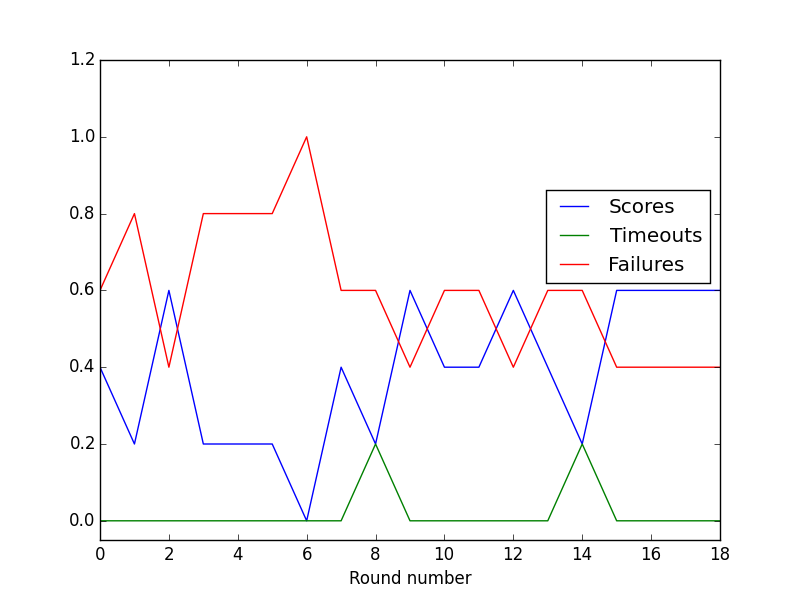
\includegraphics[width=\columnwidth]{figures/scores_coordinated_rest.png}
\caption{$< 15$ (6 teams)}
\label{fig:scores_coordinated_rest}
\end{subfigure}%
\begin{subfigure}{.5\textwidth}
\centering
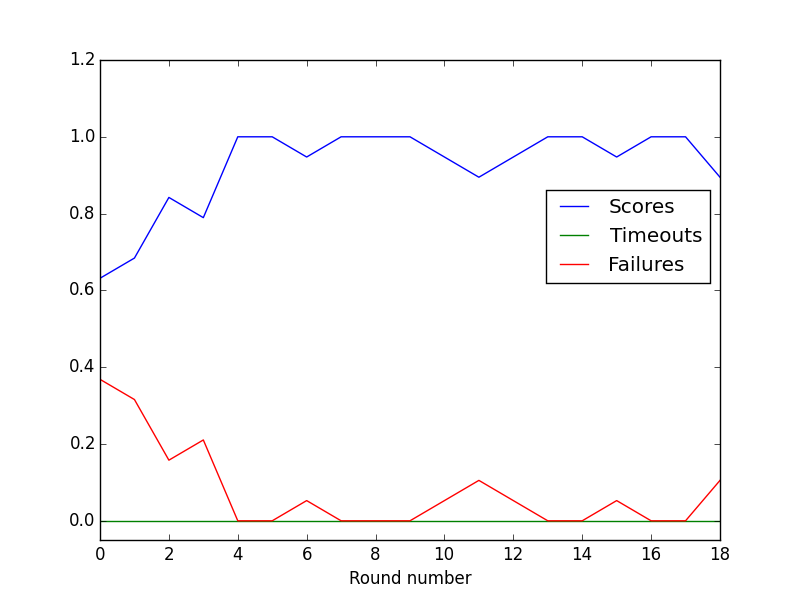
\includegraphics[width=\columnwidth]{figures/scores_coordinated_15.png}
\caption{$>= 15$ points (19 teams)}
\label{fig:scores_coordinated_15}
\end{subfigure}
\caption{Fraction of joint scores, coordination failures and round timeouts vs round number for the coordinated match group}
\label{fig:scores_coordinated}
\end{figure}

\begin{figure}
\centering
\begin{subfigure}{.5\textwidth}
\centering
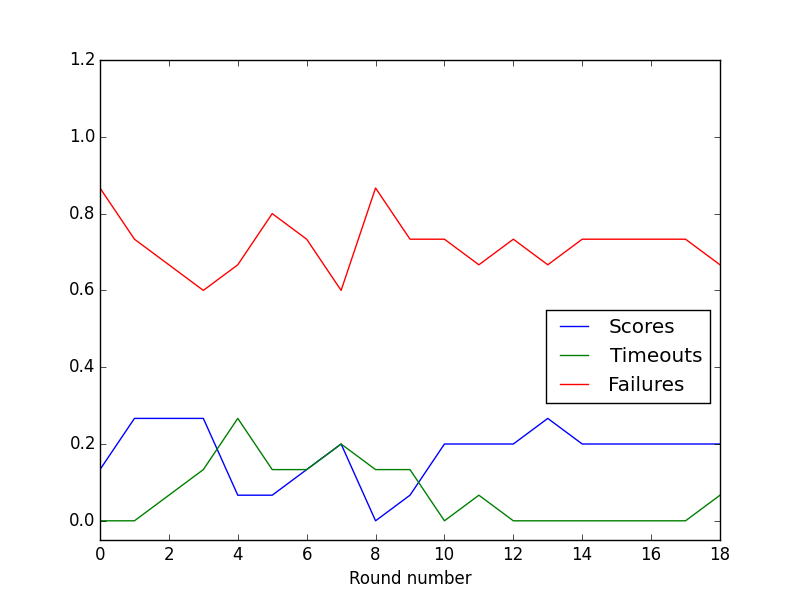
\includegraphics[width=\columnwidth]{figures/scores_uncoordinated_rest.png}
\caption{$< 15$ (17 teams)}
\label{fig:scores_uncoordinated_rest}
\end{subfigure}%
\begin{subfigure}{.5\textwidth}
\centering
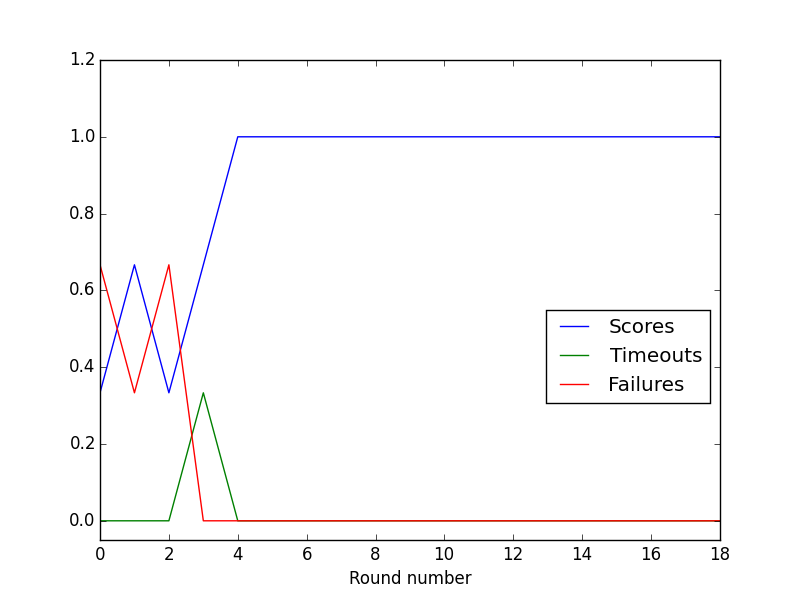
\includegraphics[width=\columnwidth]{figures/scores_uncoordinated_15.png}
\caption{$>= 15$ points (3 teams)}
\label{fig:scores_uncoordinated_15}
\end{subfigure}
\caption{Fraction of joint scores, coordination failures and round timeouts vs round number for the uncoordinated match group}
\label{fig:scores_uncoordinated}
\end{figure}


Another measure of team cooperation is the number of turns required to complete a round. Figure~\ref{fig:lengths_coordinated} and figure~\ref{fig:lengths_uncoordinated} show plots of the number of turns per round for matches with team-reasoning and with independent reasoning.

While each plot shows a lower trajectory length initially, it corresponds to lower success from figures~\ref{fig:scores_coordinated} and ~\ref{fig:scores_uncoordinated}. All matches experienced an initial increase in number of turns, but for the most cooperative teams, it quickly returns to a steady state. In the team reasoning matches, less cooperative teams experienced periodic bouts of uncoordinated rounds.

Though there were only three teams classified as cooperative in the independent reasoning group, they exhibited a more exaggerated version of the cooperative teams in the team reasoning study, suggesting that the behavior of fully cooperative teams in a more open setting will exhibit similar behaviors. For both groups of independent reasoning teams, the initial rise in the number of turns is significantly exaggerated over the team-reasoning group. 


\begin{figure}
\centering
\begin{subfigure}{.5\textwidth}
\centering
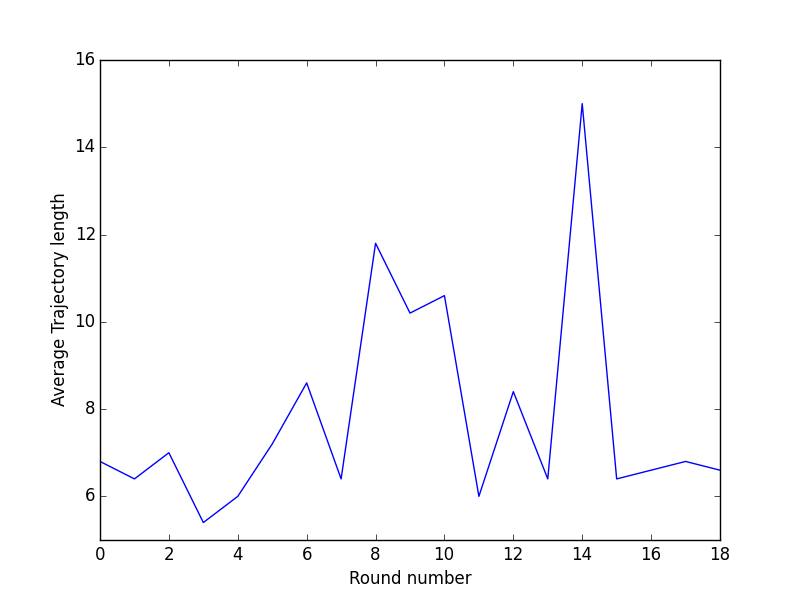
\includegraphics[width=\columnwidth]{figures/lengths_coordinated_rest.png}
\caption{$< 15$ points (6 teams)}
\label{fig:lengths_coordinated_rest}
\end{subfigure}%
\begin{subfigure}{.5\textwidth}
\centering
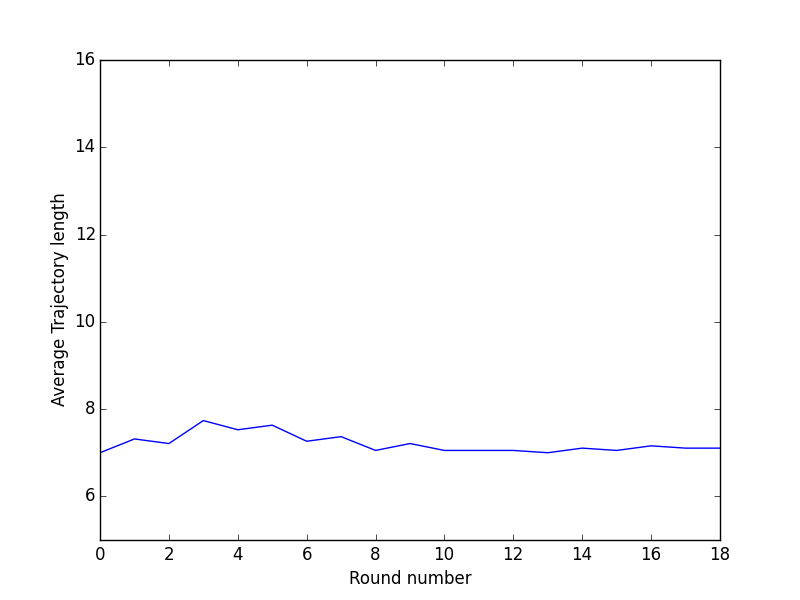
\includegraphics[width=\columnwidth]{figures/lengths_coordinated_15.png}
\caption{$>= 15$ points (19 teams)}
\label{fig:lengths_coordinated_15}
\end{subfigure}
\caption{Average number of turns per round vs round number for the team reasoning group}
\label{fig:lengths_coordinated}
\end{figure}

\begin{figure}
\centering
\begin{subfigure}{.5\textwidth}
\centering
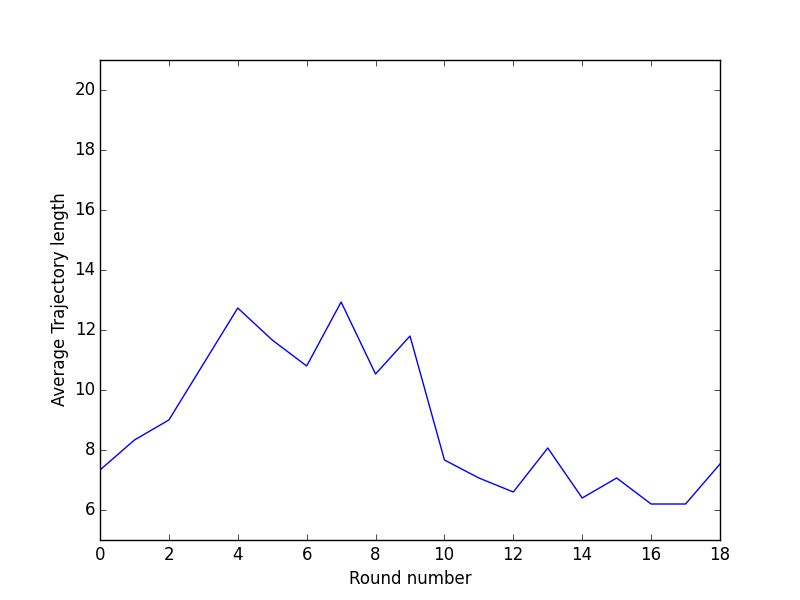
\includegraphics[width=\columnwidth]{figures/lengths_uncoordinated_rest.png}
\caption{$< 15$ points (17 teams)}
\label{fig:lengths_uncoordinated_rest}
\end{subfigure}%
\begin{subfigure}{.5\textwidth}
\centering
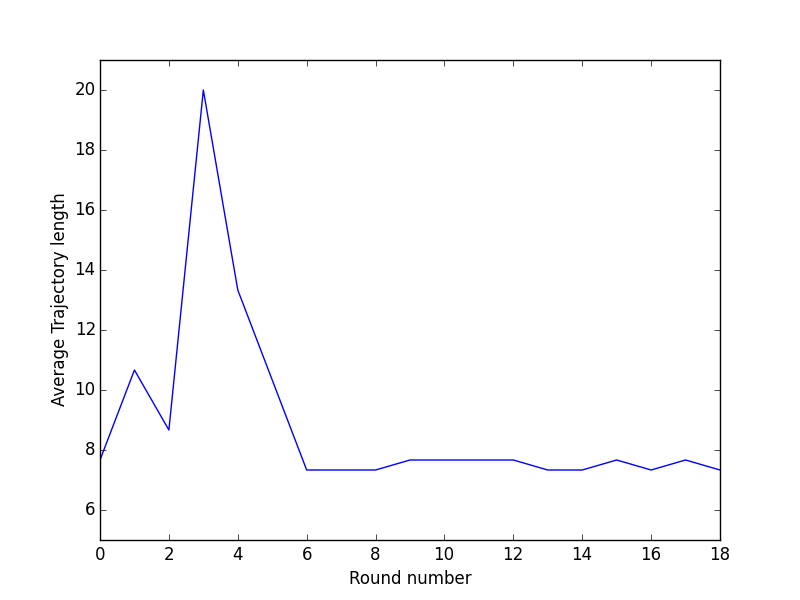
\includegraphics[width=\columnwidth]{figures/lengths_uncoordinated_15.png}
\caption{$>= 15$ points (3 teams)}
\label{fig:lengths_uncoordinated_15}
\end{subfigure}
\caption{Average number of turns per round for the independent reasoning match group}
\label{fig:lengths_uncoordinated}
\end{figure}

